We demonstrate efficacy and efficiency of our moment matching
variational MI estimators in a range of experiments beginning with a
Gaussian mixture model (\SEC\ref{sec:gmm}).  We then evaluate two
implicit likelihood models: one arising from the non-closed-form
marginalization of nuisance variables in a GLM
(\SEC\ref{sec:extrapolation}), and the other is a simulation-based SIR
epidemiology model (\SEC\ref{sec:sir}).  In all cases we find that the
proposed moment matching estimators offer substantial computational
speedups while achieving identical MI bounds and approximations to
existing methods.

%% A variety of experiments are used to demonstrate the efficiency of the 
%% Moment Matching of the Implicit Likelihood approximation compared to a 
%% variety of other approaches. The experiments chosen are joint 
%% multivariate Gaussian Mixture Model, and implicit extrapolation setting,
%% and SIR parameter estimation. We demonstrate two major takeaways. First, 
%% Moment Matching is substantially faster than Gradient based approaches 
%% for finding optimal variational distributions and second, we show that 
%% the Implicit Likelihood approximation does not sacrifice accuracy of 
%% approximation compared to Variational Posterior or Variational Marginal, 
%% which assumes exact marginal entropy or exact posterior calculation, 
%% respectively.

% \subsection{A/B Test}
% \begin{figure*}[!htb]
    \centering
    \subfigure[MI by Decision]{
    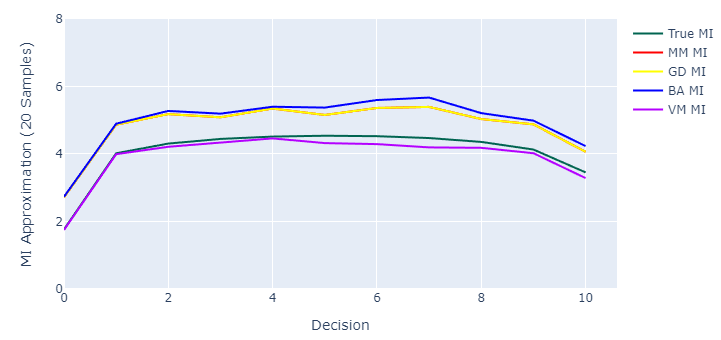
\includegraphics[width=.48\textwidth]{ABMI20.png}
    }
    \subfigure[Gradient Step Convergence]{
    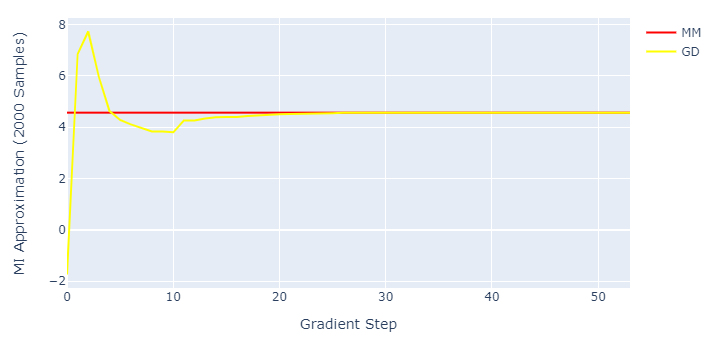
\includegraphics[width=.47\textwidth]{ABGDStep.png}
    }
    \caption{\textbf{A/B Test} for $11$ decisions of assigning $10$ participants to $2$ groups. Because the method is Gaussian linear, each model converges to the true Mutual Information. (a) $20$ samples were used to compute the mutual Information for each decision (b) This plot shows the convergence of the Gradient Descent approach approximation with respect to the number of Gradient Steps. Notice that the Gradient step converges to the Moment Matching Solution but takes $~50$ steps. The Moment Matching reaches this end convergence immediately without needing to do multiple evaluations.}
    \label{fig:ABDGStep}
    \end{figure*}
    
    We consider the classical A/B test with a Gaussian linear model. The experiment 
    in this case is where $D$ participants are chosen to be split into two 
    groups, $A$ and $B$. The design is the choice of the group size, $d_A$ for 
    group $A$ and $d_B=N-d_A$ for group $B$. Each participant then has a measured 
    continuous response $y$. The Bayesian model is a Gaussian linear as follows.
    \begin{equation}
    x\sim N(0,\Sigma_x)\hspace{2em} y|x,d \sim N(D_dx,I)\hspace{2em}\Sigma_x = \begin{bmatrix}
    10^2 & 0 \\
    0 & 1.82^2
    \end{bmatrix}
    \end{equation}
    where $D_d$ is the design matrix of size $D\times 2$ with the first $d_A$ rows 
    as $(1,0)$ and the remaining as $(0,1)$ to signify group assignments. For this 
    experiment, we will us $D=10$ participants.\\
    For variational distribution, we assumed linear multivariate gaussians from 
    the Exponential Family for both the marginal and likelihood. To evaluate each 
    approximation, $N$ samples are drawn from the prior and then the posterior 
    as $x_n\sim p(x)$ and $y_n\sim p(y|x=x_n)$.\\
    
    Figure \ref{fig:ABDGStep} shows the evaluations of Moment Matching, Gradient 
    Descent, Variational Posterior, and Variational Marginal to the true Mutual 
    Information $N=20$ Sample Points. Notice, the Moment Matching and Gradient 
    Descent Approach both match for each decision evaluation as expeceted. In 
    Figure  \ref{fig:ABDGStep}, we compare the Mutual Information evaluation of 
    Moment Matching to that of Gradient Descent with respect to gradient steps. 
    Notice that Gradient Descent approaches the Moment match solution but take 
    approximately K step before it has leveled out.\\
    
    Another important property to observe from the Figure \ref{fig:ABDGStep} is 
    that the theoretical bound have been swapped for Varaitional Posterior and 
    Variational Marginal distributions, that is Variational Marginal should be 
    an upper bound but is a lower bound and vice-versa. This is due to a bias 
    introduced from finite sample plug in estimators. It is easily shown 
    that $\E[\hat{\Sigma}]=\frac{n+1}{n-1}\Sigma$. So in this case where our 
    variational distributions are the same family as the target distributions 
    (Gaussian), the error bound from Gibbs' inequality is less than that of the 
    introduced bias and the bound swaps. For examples where the target distribution 
    is not a Gaussian, the bias tends to be negligible compared to the approximation 
    bound.\\
    
    For further analysis, Figure \ref{fig:ABConvergence}, the convergence rate and 
    time of each method is shown for the decision with the maximum Mutual 
    Information ($d=5$) with respect to the number of samples taken. We notice after 
    a few hundred samples, all of the methods have converged to the true Mutual 
    Information. We also see that for computation time, every method is orders of 
    magnitude faster than that of the Gradient Descent. We will see that as the 
    dimensionality of the problem increases, the speed of Moment Matching will be 
    highlighted in comparison to Variational Marginal and Variational Posterior.
    
    \begin{figure*}[!htb]
    \centering
    \subfigure[MI Convergence]{
    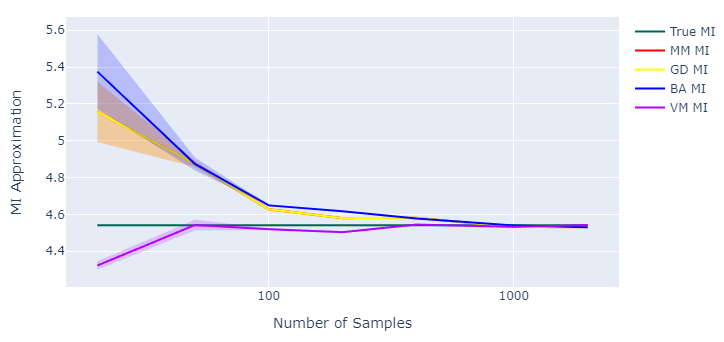
\includegraphics[width=.48\textwidth]{ABConverge.png}
    }
    \subfigure[Computation Time]{
    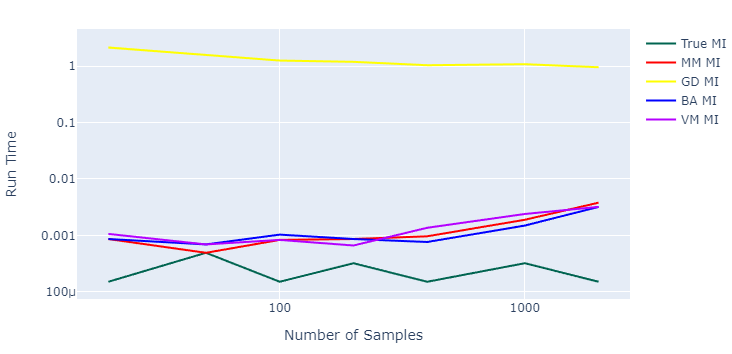
\includegraphics[width=.47\textwidth]{ABTime.png}
    }
    \caption{\textbf{A/B Test Mutual Information Estimation} for $11$ decisions of assigning $10$ participants to $2$ groups. Because the method is Gaussian linear, each model converges to the true Mutual Information. (a) The convergence of MI with respect to the number of samples drawn is plotted for the maximum MI decision ($d=5$) (b) The run time of each method is plotted for the number of samples for the maximum MI decision ($d=5$). Note that Moment Matching and Gradient Descent Match in approximation Value however Moment matching save orders of magnitude in computation time. }
    \label{fig:ABConvergence}
    \end{figure*}

\subsection{Multivariate Gaussian Mixture Model}\label{sec:gmm}
GMMs are pervasive in statistics due to their universal approximation
properties, yet calculating MI for a GMM is notoriously
challenging~\cite{huber2008entropy}.  In this section we extend the
two-dimensional example (\FIG\ref{fig:GMMex}) to high-dimensional
GMMs.  We simulate a bivariate GMM,
\begin{equation}
  p(x,y) = \omega \Ncal(m_0, \Sigma_0) + (1-\omega) \Ncal(m_1, \Sigma_1)
\end{equation}
with $\omega \in [0, 1]$ and dimensions $X \in \mathbb{R}^{100}$ and
$Y \in \mathbb{R}^{200}$.  We use this setting to demonstrate
efficient MI estimation even in very high-dimensional distributions.

\FIG\ref{fig:LargeGMMConvergence} shows substantial speedups in
runtime (left) for all methods as compared to gradient optimizatoin
(center).  Notice that GD takes approximately 2000 gradient steps to
converge for $5,000$ samples whereas moment matching found this
solution immediately, independ of any gradient steps.  As per our
theoretical results we find that $\Iml$ always lies between the MI
upper bound $\Imarg$ and lower bound $\Ipost$ with $\Imarg$ being most
accurate estimator in this model (right).
\begin{figure*}[t]
  \centering
  \begin{tabular}{ccc}
    \hspace*{-4mm}\subfigure[Computation Time]{
    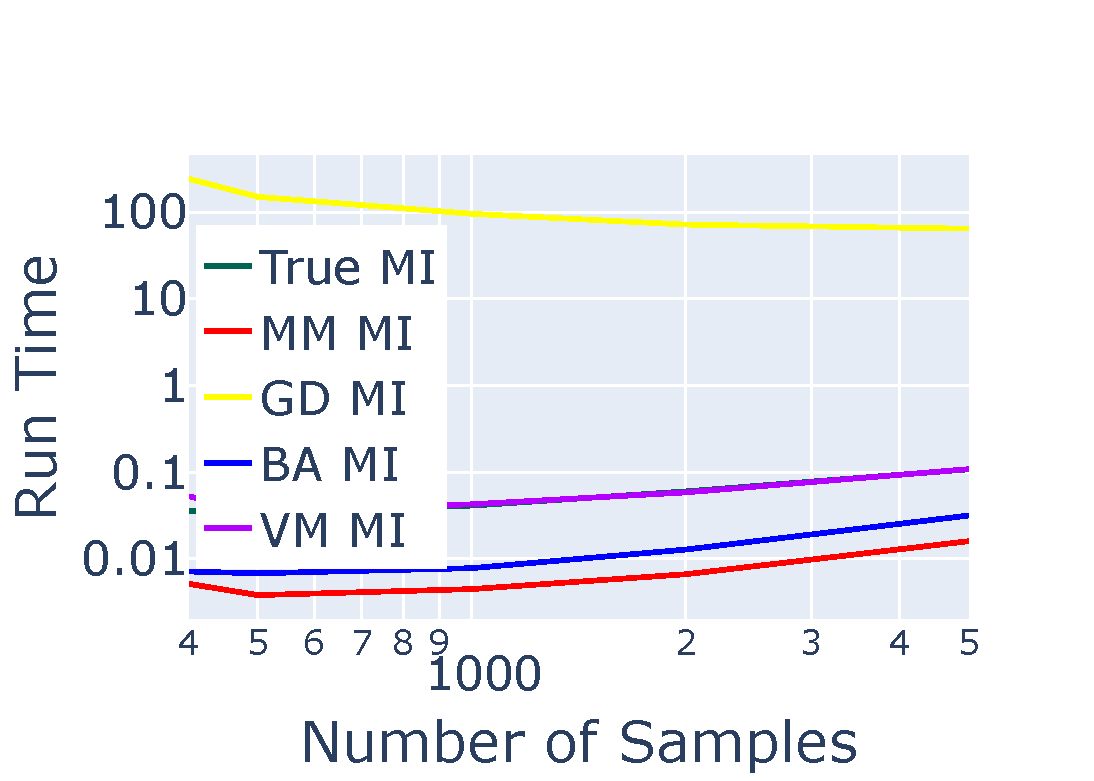
\includegraphics[width=.36\textwidth]{LargeGMMTime.pdf}
    }
    \hspace*{-6mm}\subfigure[GD Convergence]{
        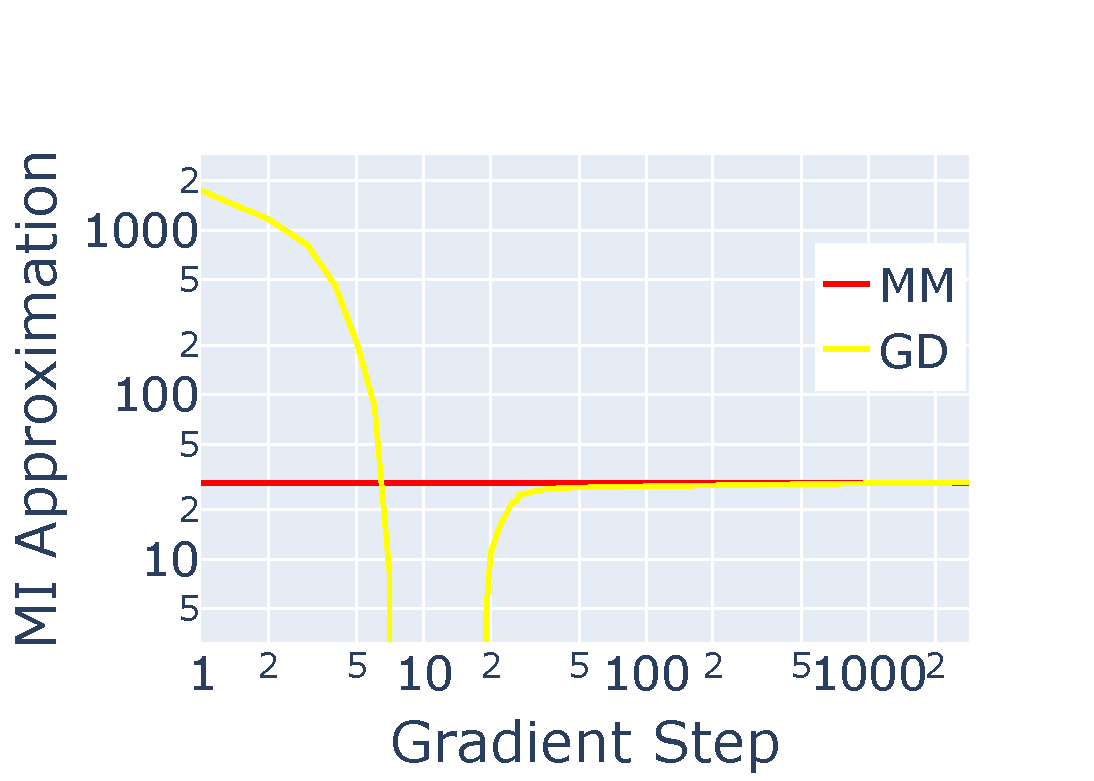
\includegraphics[width=.36\textwidth]{GMMGDStep.pdf}
    }    
    \hspace*{-6mm}\subfigure[MI Convergence]{
    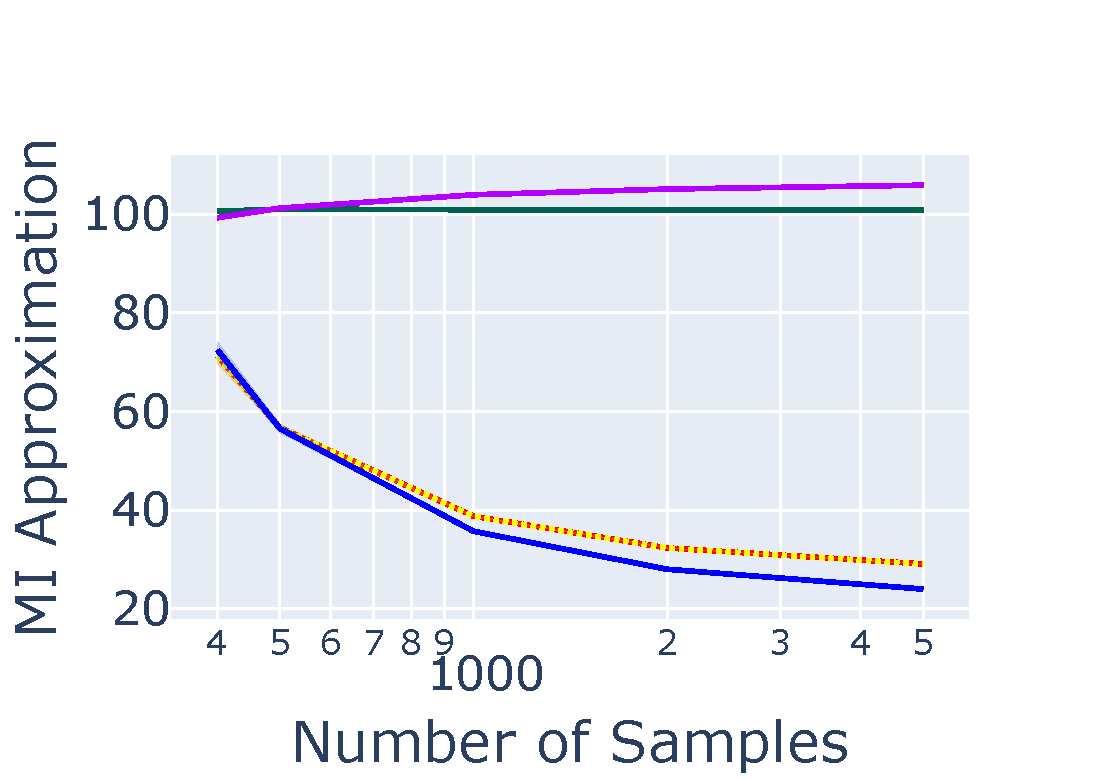
\includegraphics[width=.36\textwidth]{LargeGMMConverge.pdf}
    }
  \end{tabular}
    \caption{\small\textbf{High-dimensional Bimodal GMM.} Moment
      matching estimates have orders of magnitude lower computation as
      a function of sample size (a).  As per our theoretical analysis,
      our moment-matching solution to $\Iml$ achieves the same
      estimate while avoiding gradient iterations (b).  In this model
      we see that $\Imarg$ yields the most accurate estimates.  ``True
      MI'' is calculated via Monte Carlo estimation with exact
      evaluation of the model probabilities.}
    \label{fig:LargeGMMConvergence}
    \end{figure*}

%% sample convergence (right) for each method. We see that each
%% approximation satisfies the theoretical bounds discussed, with
%% $\Ipost$ as a lower bound, $\Imarg$ as an upper bound, and $\Iml$
%% lying inbetween. We can observe the computation times in this high
%% dimensional case. The true MI is more computationally intensive in
%% this scenario so we see that Moment Matching is slighly faster than
%% computing $\Imarg$ and $\Ipost$.

%% A synthetic model is constructed for explicit comparing of methods. In these 
%% experiments, a multivariate Gaussian Mixture Model with $K$ modes, latent 
%% variable dimension $D_x$, and observation variable dimension $D_y$ , is generated 
%% as the joint distribution. Samples can be directly drawn from the prior and 
%% then the posterior as $x_n\sim p(x)$ and $y_n\sim p(y|x=x_n)$. Since the true 
%% distributions are known, the true entropy can be numerically calculated using 
%% these samples. We will compare each of the methods to this numerical calculation.\\

%% The GMM we will consider will have high dimensions, with $K=2$, $D_x=100$ 
%% and $D_y = 200$. The purpose of this will be to emphasis the efficiency of 
%% calculating MM approximation over the Varaitional Marginal, Variational Posterior,
%% and especially over Gradient Descent. \\

%% Most importantly, moment matching is orders of magnitude faster than
%% computing the Gradient Descent approach for the exact same
%% approximation. To emphasis this result, consider the convergence of
%% gradient descent in Figure \ref{fig:LargeGMMConvergence}
%% (right). 

%% Using Moment Mathcing for $\Iml$, notice that we get similar quality approximations
%% to MI while saving drastic compution time. In a scenario with even higher 
%% dimensionality or a large domain of decisions, the computational speed up of Moment
%% Matching is drastic compared to $\Imarg$, $\Ipost$, and especially $\hat{I}_{NMC}$.


% \begin{figure*}[!htb]
%     \centering
%     \subfigure[MI Convergence]{
%     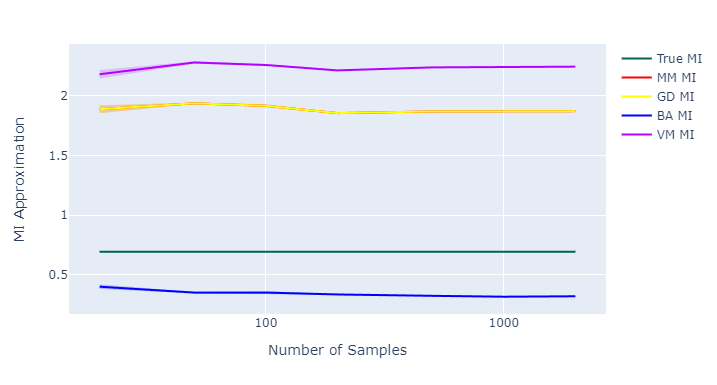
\includegraphics[width=.34\textwidth]{GMMMI.png}
%     }
%     \subfigure[Computation Time]{
%     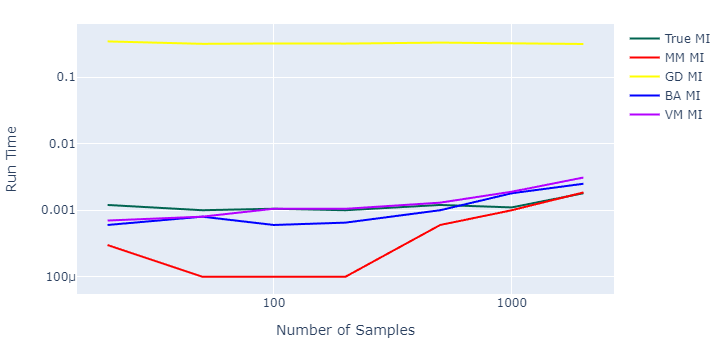
\includegraphics[width=.34\textwidth]{GMMTime.png}
%     }
%     \subfigure[Samples]{
%     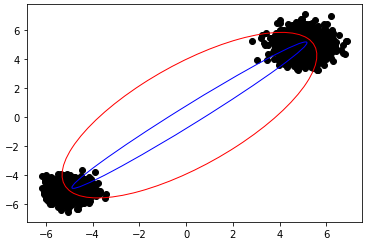
\includegraphics[width=.26\textwidth]{GMMSample.png}
%     }
%     \caption{\textbf{Gaussian Mixture Model Mutual Information Estimation} A Guassian Mixture model with 2 modes and Dimensions of Latent Variable, $X$, and Observation Variable $Y$, both being $1$. (a) The convergence of MI with respect to the number of samples drawn is plotted (b) The run time of each method is plotted for the number of samples. (c) The plotted samples drawn with an overlayed Moment Matched Gaussian Variational Approximation and an "Oracle" Gaussian approximation that matches the true Mutual Information. Variational Marginal is and upper bound, Variational Posterior is a lwoer bound, and MM/GD is a closer upper bound.}
%     \label{fig:GMMConvergence}
%     \end{figure*}
% Likewise, we can compute and "oracle" variational distribution which learns 
% it parameters by minimizing the absolute difference in the numerical Mutual 
% Information to the Implicit Likelihood approximation. This will be used to 
% qualitatively compare against the learned moment matching distribution.
% The first GMM we will consider will have $K=2$, $D_x=1$, and $D_y=1$. 
% Figure \ref{fig:GMMConvergence} show the convergence rate and time of each 
% methods. Now that our model is no longer linear gaussian, we see that the bound 
% of each methods holds as the bias introduced due to the plug in estimator is 
% negligible with respect to the varitional bounds. We again notice that each 
% method is significantly faster than that of the Gradient Descent.\\

% Figure \ref{fig:GMMConvergence} shows the sampled points along with the 
% Moment Match distribution and the Oracle distribution. We notice that both 
% share many similar quantities however the Oracle is a has larger variance 
% in on direction. This is responsible for lowering the Mutual Information to 
% match the True Mutual information by creating more uncertainty in the added 
% variance. This shows where the information is lost in Moment Matching for this 
% example.\\


\subsection{Extrapolation}\label{sec:extrapolation}
\begin{figure*}[!t]
    \centering
    \hspace*{-5mm}\subfigure[MI Convergence]{
      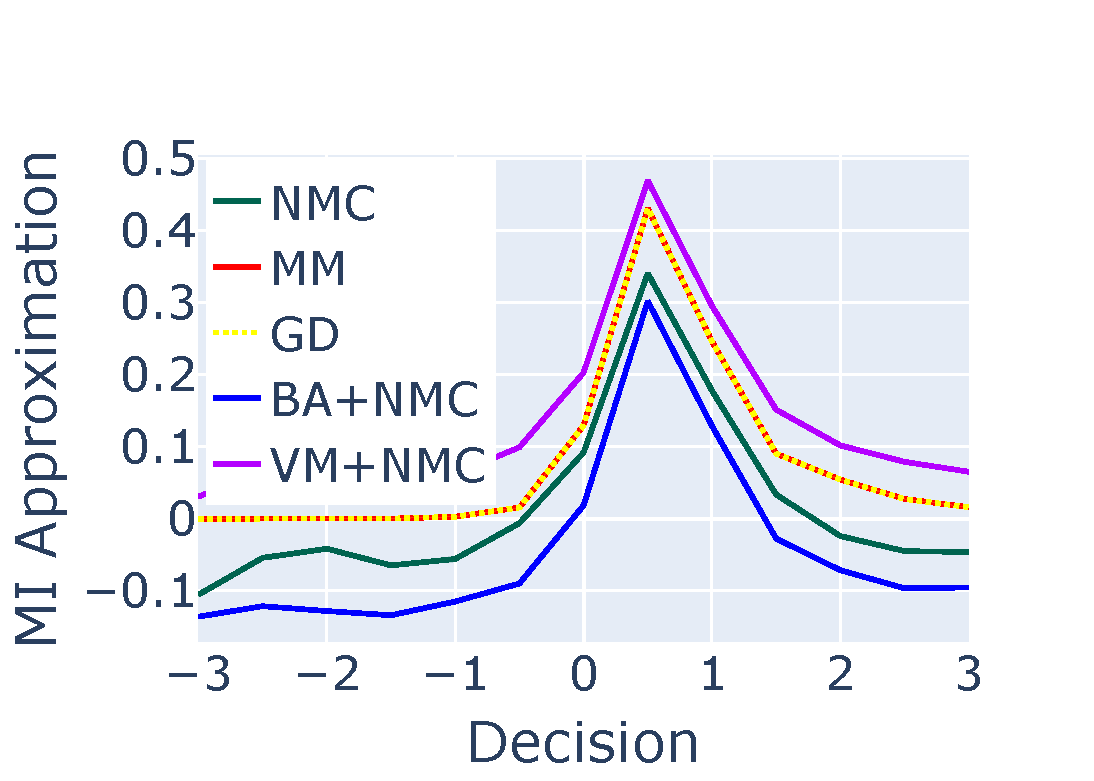
\includegraphics[width=.36\textwidth]{ExtrapolationMI.pdf}
    }
    \hspace*{-7mm}\subfigure[Computation Time]{
      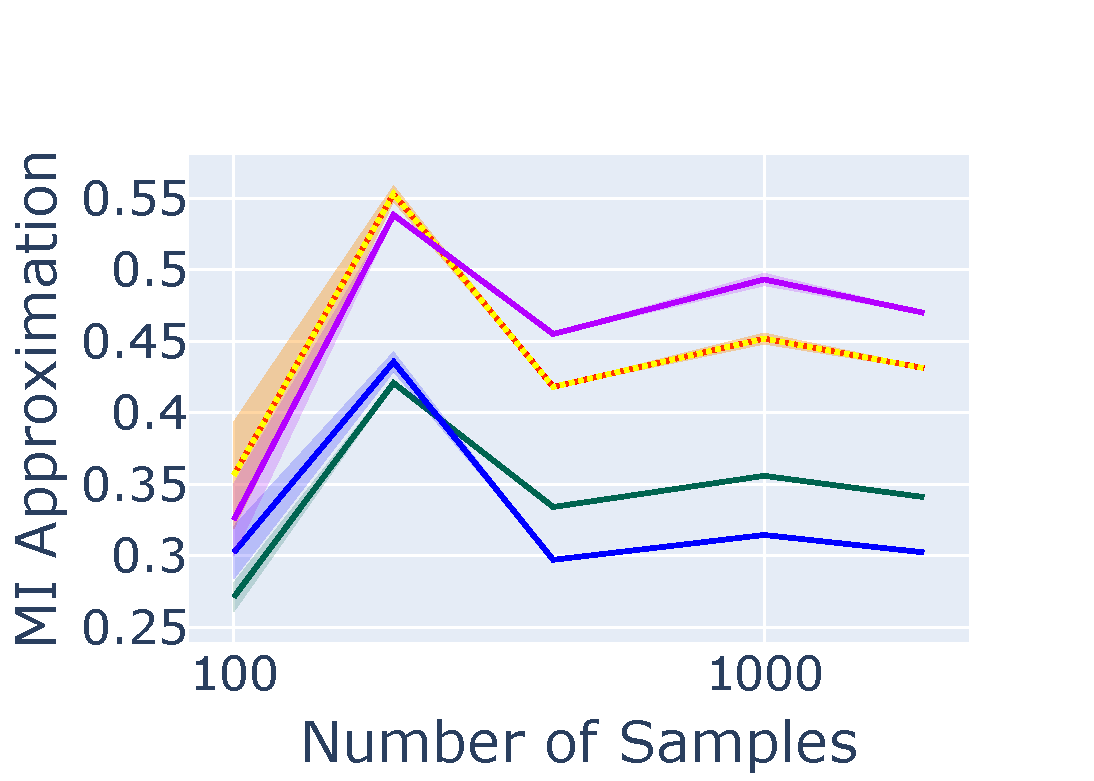
\includegraphics[width=.36\textwidth]{ExtrapolationConverge.pdf}
    }
    \hspace*{-7mm}\subfigure[Samples]{
      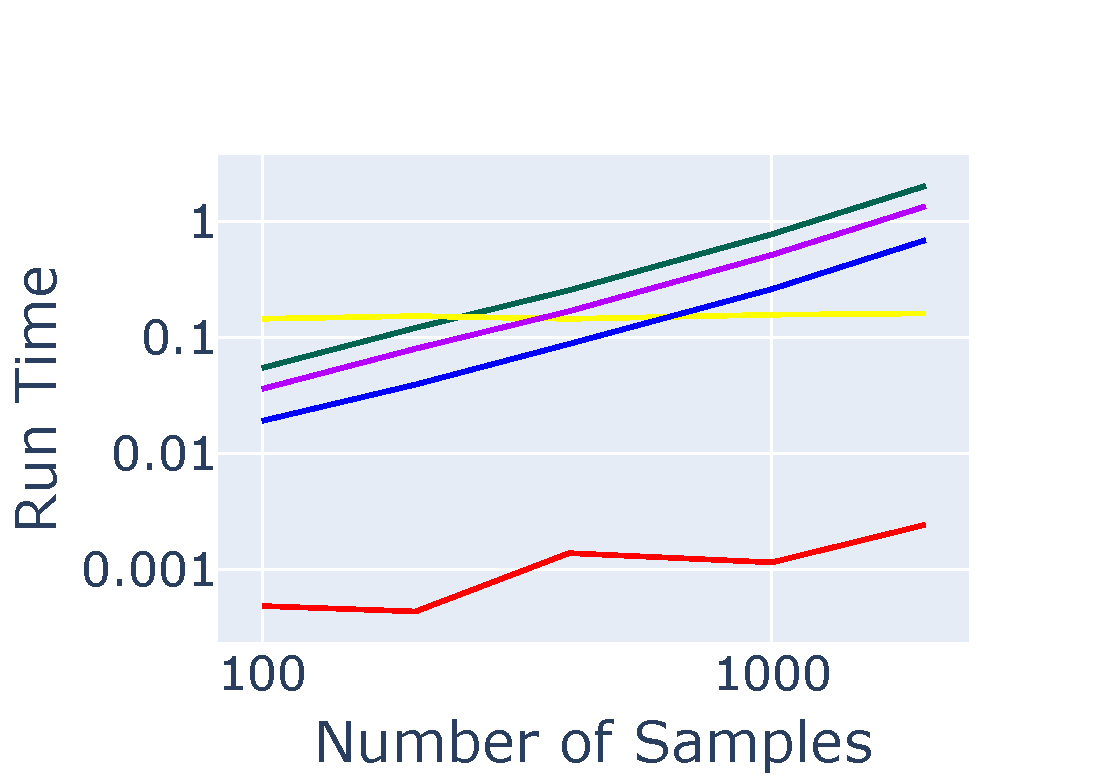
\includegraphics[width=.36\textwidth]{ExtrapolationTime.pdf}
    }
    \caption{\small \textbf{Extrapolation} (a) The MI for decisions $d
      \in [-3,3]$ with variances $\sigma_x^2 = 3$, and $\sigma_y^2=1$
      for each approximation with 4000 samples is plotted with $d=.5$
      being the maximum. Note the negative bias resulting from
      NMC. (b) The convergence rate versus samples is plotted at
      maximum decision ($d=.5$) (c) The run time for each method is
      plotted with moment matching being orders of magnitude faster than
      any other method.}
    \label{fig:Extrapolation}
\end{figure*}

We adapt the following experiment from Foster et
al.~(\citeyear{Foster2019}) intended to evaluate the implicit
likelihood MI estimator $\Iml$ (or $\hat{I}_{m+\ell}$).  Labeled
information, $y$, from a subset of the design space is be used to
predict labels at a location $x$ that can't be directly observed. The
model is as follows,
\[
 \psi\sim \Ncal(\mu_\psi, \Sigma_\psi), \quad  \theta \mid \psi \sim \Ncal\left( (X_\theta^T \psi)^2, \sigma_x^2 \right) \quad y\mid\psi,d \sim \Ncal\left( (X_d^T \psi)^2, \sigma_y^2 \right)
\]
where $X_x = (1,-\frac{1}{2})$ and $X_d = (-1,d)$.  The aim is to
choose a design $d \in \mathbb{R}$ that maximizes $I(\theta ; Y \mid
d)$.  Thus, $\psi$ is a nuisance variable that must be marginalized.
This marginalization lacks a closed-form and so the likelihood $p(y
\mid \theta)$ is implicit--it cannot be evaluated nor efficiently
sampled.  As a baseline we draw $N$ samples from the joint and use the
NMC estimator to compute entropies as:
\begin{equation}
    H(\theta)= -\int p(\theta)\log(p(\theta))dx \approx -\dfrac{1}{N}\sum_i \log\left(\dfrac{1}{N-1}\sum_{j\neq i}p(\theta_i|\psi_j)\right)
    \label{eq:NMCentropy}
\end{equation}
%% To compute each of these methods, we will sample from $x_i,y_i,\psi_i
%% \sim p(\psi)p(x|\psi)p(y|\psi,y)$ and we will need to compute a NMC
%% estimator for the $H_p(p)$ terms in $\Imarg$ and $\Ipost$ as well as
%% for a total approximation of $I(X,Y)\approx I_{NMC}(X,Y)$. To compute
%% each entropy term from samples, we use

\FIG\ref{fig:Extrapolation} summarizes the proposed estimators and
runtime.  As the theory suggests our moment matching estimators
provide substantial speedup, and we observe accurate estimates with
$\Iml$ in this model.  We emphasize that $\Imarg$ and $\Ipost$ are
infeasible due to the need to estimate model entropies in this
implicit likelihood model.  We instead augment these methods with the
NMC estimator (e.g. \EQN\eqref{eq:NMCentropy}), which is referred to
as \emph{variational NMC} in the literature~\cite{Foster2019}.
However, the finite sample bias of NMC violates expected bound
properties for few samples--see \FIG\ref{fig:Extrapolation} (center).
We include these estimators to highlight the difficulty of estimating
MI in implicit likelihood models and to emphasize their practical
limitations.

%% An issue with this approximation is that despite it being consisent, it is biased
%% and the bias decays slowly (Zheng, 2018). When we observe Figure
%% ~\ref{fig:Extrapolation}(a)(b), we notice that the NMC is negative for some 
%% values of $d$. $I(X,Y)\geq0$ so this is the effect of the bias. Likewise, since 
%% the Variational Posterior and Variatoinal Marginal use entropy terms computed
%% using the NMC, they too are biased. However, we do notice that we maintain the 
%% ordering of the approximators from Lemma~\ref{lemma:MIOrder}.\\
%% From the experiment, we see that the optimal decision is when $d=.5$. This makes
%% intuitive sense for our problem as $X_x=(1,-\frac{1}{2})$ and 
%% $X_d = (-1,\frac{1}{2})$ which implies that they are highley negatively 
%% correlated, giving infromation about one another. As for the run time in (c), we
%% notice that Moment Matching is uniformaly faster than any other method by a few
%% orders of magnitude. Also, after approximatley 500 samples, the gradient decsent
%% based method becomes computationally cheaper than the NMC methods.\\
%% From this experiment, we see that moment matching provides a qualitatively good 
%% estimation as any other method while simulateously saving orders of magnitude in
%% computation time.\\


\subsection{SIR Epidemic Model}\label{sec:sir}
\begin{figure*}[t!]
  \centering
  \hspace{-8mm}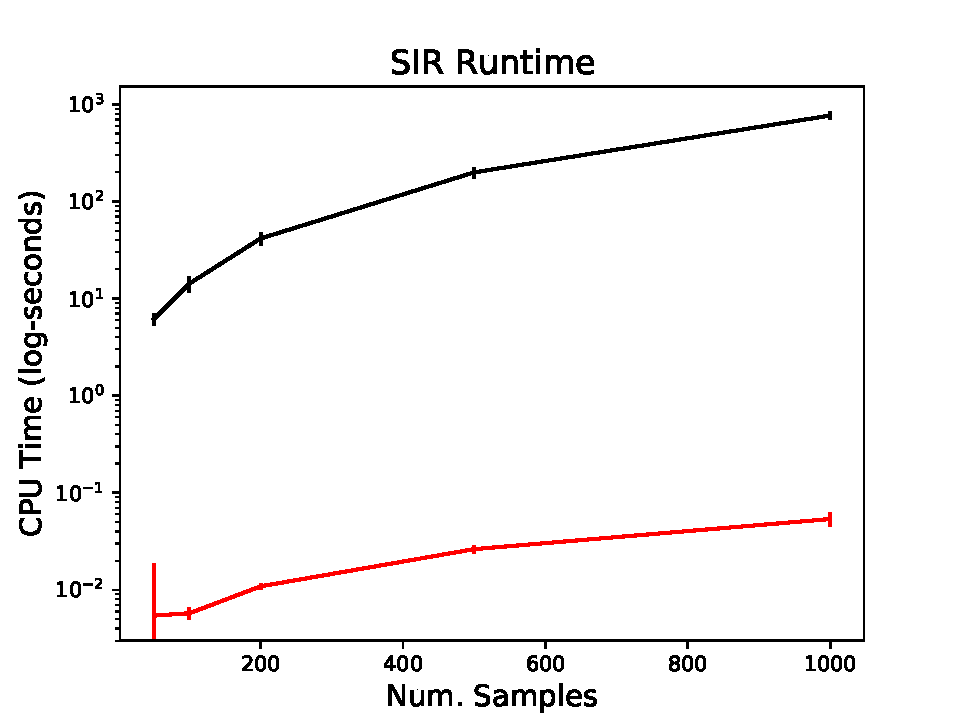
\includegraphics[width=0.28\textwidth]{sir_runtime_benchmark}
  \hspace{-4mm}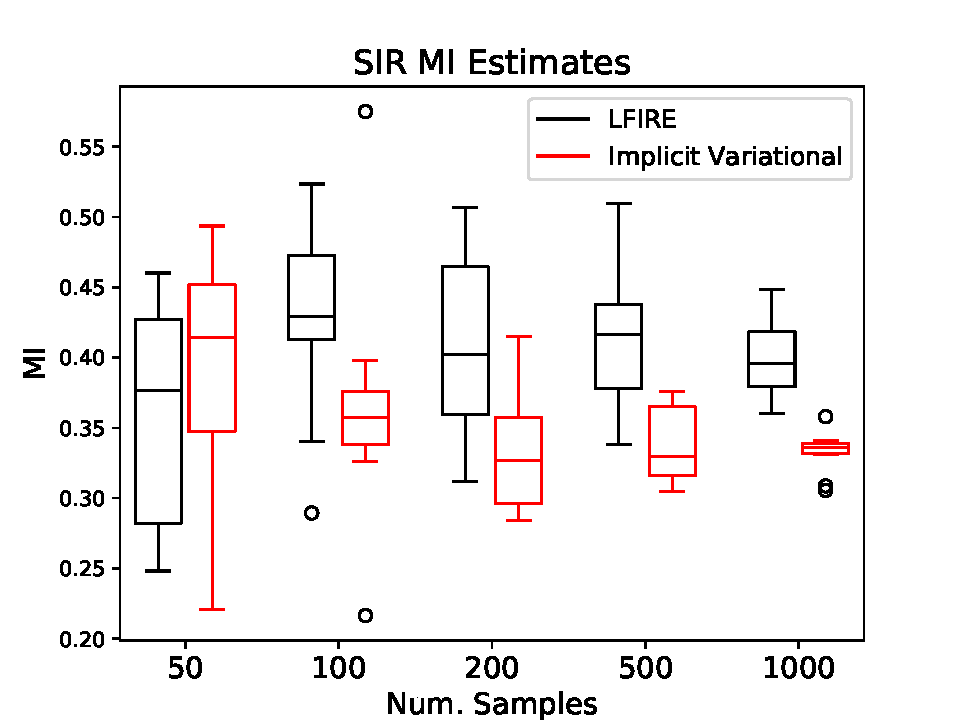
\includegraphics[width=0.28\textwidth]{sir_utility_benchmark}
  \hspace{-4mm}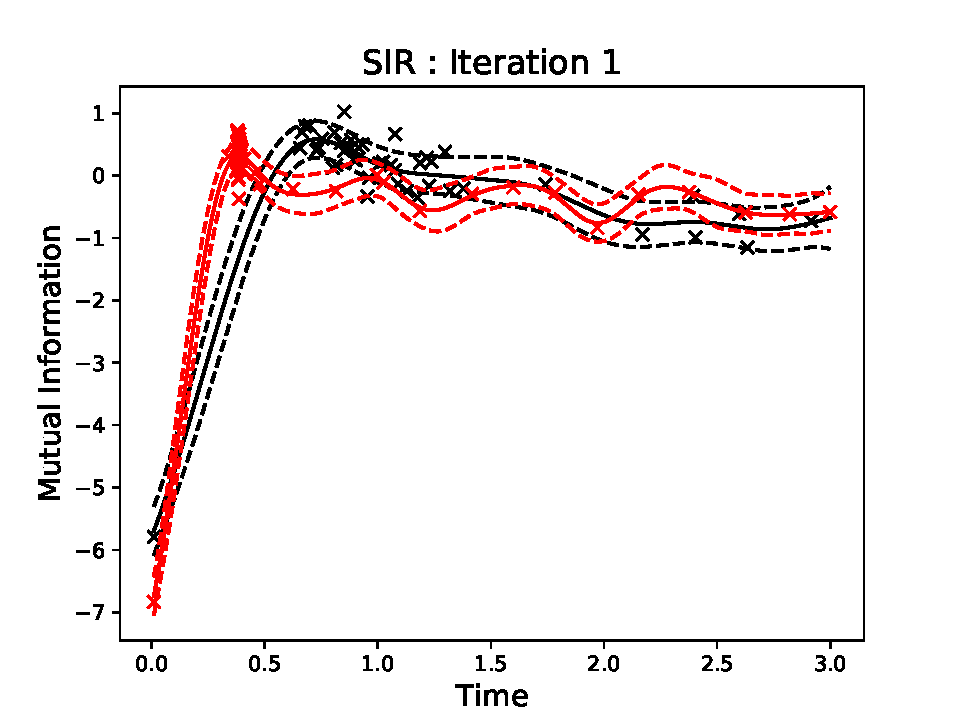
\includegraphics[width=0.28\textwidth]{sir_500p_K3_iter1}
  \hspace{-4mm}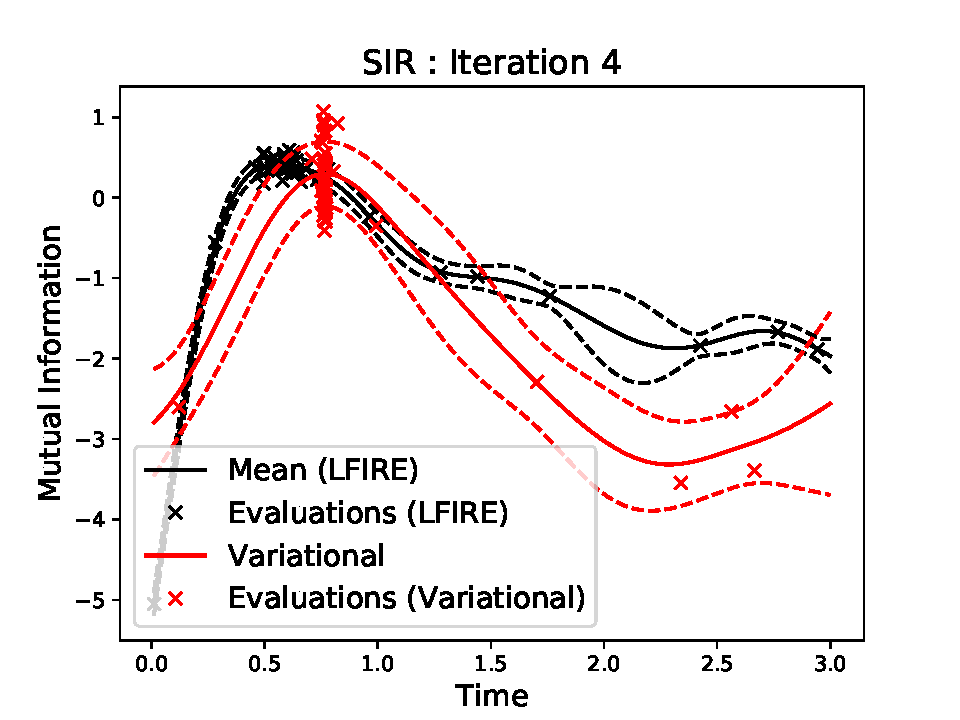
\includegraphics[width=0.28\textwidth]{sir_500p_K3_iter4}
  \caption{\small \textbf{SIR Sequetial Design.} Left plots show benchmark
    time and utility evaluation between LFIRE and the Variational
    estimator for a fixed design ($d=1.0s$) over 10 runs each at a
    range of sample sizes.  The variational estimator is orders of
    magnitude more efficient (\emph{left}) and shows lower variance at
    each sample (\emph{center-left}).  The first (\emph{center-right})
    and fourth (\emph{right}) sequential BED iterations yield
    comparable designs between both methods (GP posterior MI shown).}
  \label{fig:sir_results}
\end{figure*}

\paragraph{The SIR model} 
describes the time-evolution of infection in a fixed
population~\cite{kermack1927contribution, allen2008introduction}.  At
each time $t$ the population is divided into three components:
\emph{susceptible} $S(t)$, \emph{infected} $I(t)$, and
\emph{recovered} $R(t)$ according to the time-series,
\begin{align}
  S(t + \Delta_t) &= S(t) - \Delta I(t) \label{eq:s} \\
  I(t + \Delta_t) &= I(t) + \Delta I(t) - \Delta R(t) \\
  R(t + \Delta_t) &= R(t) + \Delta R(t) \label{eq:r}
\end{align}
\begin{wrapfigure}{r}{0.3\textwidth}
  \vspace*{-5mm}
  \centering
  \hspace*{-5mm}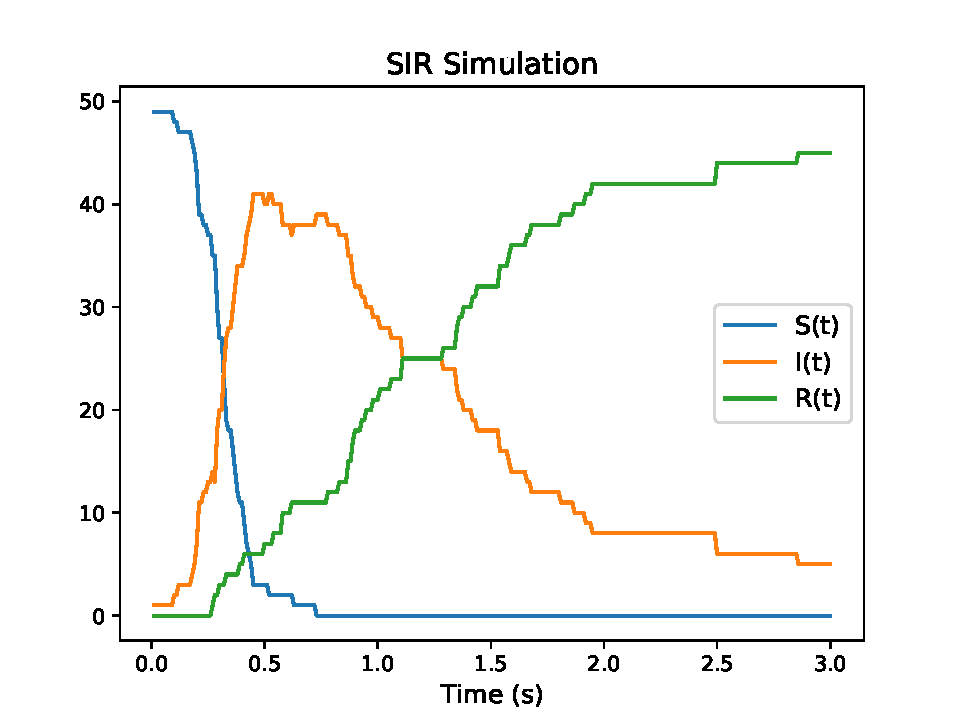
\includegraphics[width=0.35\textwidth]{sir_sim_beta_0p14_gamma_0p01}  
  \caption{\small SIR model simulation for $\beta = 0.14,
    \gamma=0.01$.}
  \vspace*{-5mm}
  \label{fig:sir_sim}
\end{wrapfigure}
At each time the change in infected $\Delta I(t)$ and recovered
$\Delta R(t)$ are Binomially distributed,
\[
  \Delta I(t) \sim \text{Binomial}\left(S(t), \frac{\beta
    I(t)}{N}\right), \quad
  \Delta R(t) \sim \text{Binomial}(I(t), \gamma)
\]
with unknown random parameters $\beta, \gamma \sim
\text{Uniform}(0,0.5)$.  Our simulations use a fixed discrete time
interval $\Delta_t = 0.01$ with a population $N=50$ and boundary
conditions $S(t=0) = N-1$, $I(t=0)=1$, and $R(t=0) =
0$. See \FIG\ref{fig:sir_sim} for an example of the SIR simulation.


\paragraph{Sequential Design} We select a time $t > 0$ with maximal
information about the parameters $\beta, \gamma$ as in, \mbox{$\argmax_t \, I\left(\{\beta, \gamma\} ; \{S(t),
I(t)\} \right)$}.
%% Early and late
%% stages are uninformative, since the population is largely uninfected
%% or recovered.  
We ignore $R$ in the MI quantity since it is deterministic via: $R(t)
= N - I(t) - S(t)$.  After choosing a time $t^*$ we observe $S(t^*) =
s$, $I(t^*) = \iota$, and $R(t^*) = r$.  In stage $K$ of sequential
(greedy) design we condition on $K-1$ previously-chosen times $t^*_1,
\ldots, t^*_{K-1}$ and their resulting observations $\{s_1^{K-1},
\iota_1^{K-1}\}$, denoted by the ``history'' set $\mathcal{H}_{K-1}$.  The
$K^{\text{th}}$ time is chosen to maximize,
\begin{equation}\label{eq:mi_sir}
  t_K^* = \argmax_{t > 0} \; I\left(\{\beta, \gamma\} ; \{S(t),
  I(t)\} \mid \mathcal{H}_K \right).
\end{equation}
Optimizing \EQN\eqref{eq:mi_sir} is complicated since the SIR lacks an
explicit likelihood \mbox{$p(S(t), I(t), R(t) \mid \beta, \gamma)$}--it is
defined implicitly through simulation of
\EQNS\eqref{eq:s}-\eqref{eq:r}.  Existing design approaches to
sequential design in this model~\cite{kleinegesse2021sequential} rely
on LFIRE~\cite{thomas2022likelihood} estimates of the ratio
$\frac{p(S, I, R \mid \beta, \gamma)}{p(S, I, R)}$ for calculating MI
in \EQN\eqref{eq:mi_sir}.

\paragraph{Fast and accurate variational estimates.} We compare our moment-matched
$\hat{I}_{m+\ell}$ MI estimator to the LFIRE estimator.  For
sequential design we use the implementation of Kleinegesse et
al.~(\citeyear{kleinegesse2021sequential}) which estimates MI based on
importance weighted expectations of the LFIRE ratio estimator.
\FIG\ref{fig:sir_results} shows that our moment matching estimates
achieve several orders of magnitude speedup (left) with comparable
estimates and reduced variance (left-center).  We note that our
estimates are based on the same samples as those used in LFIRE.  In
sequential greedy design we observe comparable time-point selections
across iterations as compared to that of Kleinegesse et
al. (center-right and right).  Note that Kleinegesse et al. report
only 4 design stages since the code is prohibitively slow for further
designs.  Using our estimator it is possible to conduct many more
design iterations in a fraction of the time.




% Our simulations use a fixed discrete time interval of $\Delta_t =
% 0.01$ units.  

